\chapter{Fundamentals and State of the Art}
\label{ch:literature}

\section{Asset Administration Shells(AAS)}
The \ac{AAS} is one of the central concepts in the principles of Industry 4.0, 
providing a methodology for designing and implementing the digital representation 
of manufacturing process components \cite{arm2021automated}.
This section explores the fundamental concepts of the \ac{AAS}, its structure, 
and its role in enabling interoperability within Industry 4.0 ecosystems.
This section cover the specifications in \cite{plattformi40_aas_part1_v3}, \cite{plattformI40_aas_part2} that are of relevance
to this thesis.

\subsection{Basic concept of AAS}

The \ac{AAS} is a standardized digital representation of an asset,
which can be a physical or virtual entity within an industrial environment.
It serves as a cornerstone for achieving interoperability and seamless communication
of the asset with other components in the Industry 4.0 ecosystem \cite{idta2023metamodel}.
Together with the asset it represents, the \ac{AAS} forms the so-called 
\ac{I4.0} Component (I4.0-Component), as illustrated in Figure~\ref{fig:i4component}.
The asset can be any physical or non-physical entity that has value for an organization, 
including production systems, equipment, machines, components, products, raw materials, 
business processes, software, documents, and even human personnel \cite{idta2023metamodel}.

\begin{figure}[ht]
    \centering
    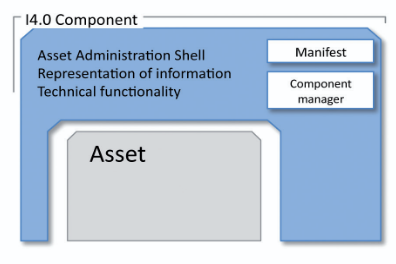
\includegraphics[width=10cm]{Images/AAS_OverViewConcept.png}
    \caption{The Industry 4.0 Component: Asset and its Administration Shell \cite{idta2023metamodel}}
    \label{fig:i4component}
\end{figure} 
At its core, the \ac{AAS} is an information model (meta model) that 
is exchanged between \ac{I4.0} components to enable interoperability \cite{plattformi40_aas_part1_v3}.
This information model could be represented as a \textit{\ac{XML}}, \textit{\ac{JSON}} or \textit{\ac{RDF}} document \cite{plattformi40_aas_part1_v3}.

The figure~\ref{fig:AAS_MetaModel} illustrates the meta model of the \ac{AAS},
which defines its structure and key components.
According to \cite{plattformi40_aas_part1_v3}, the \ac{AAS} has an \textit{Identifiable} attribute, which translate to an element
that is referable via a unique identifier.This attribute ensures that each \ac{AAS} can be distinctly identified within the Industry 4.0 ecosystem which also makes them unambiguous and easy to find.
Also it make the \ac{AAS} into an \textit{AdministrativeInformation} ,which contains information about the versioning , who created the last changes and information about the languages available in case the element contains text for translation \cite{plattformi40_aas_part1_v3}.
Also each \ac{AAS} has a \textit{HasDataSpecification} attribute, which means that it can be extended by using data specification templates , those define a named set of additional attributes that
an element may or shall have \cite{plattformi40_aas_part1_v3}.
The \ac{AAS} also has a \textit{derivedFrom} relation, which allows it to reference another \ac{AAS} from which it is derived.
This relation is useful for establishing hierarchies or relationships between different \ac{AAS}s.
The most important attribute of the \ac{AAS} is the \textit{HasSubmodel} attribute,
which indicates that the \ac{AAS} contains one or more submodels.
Submodels are modular components within the \ac{AAS} that encapsulate specific functionalities
and data related to the asset \cite{plattformi40_aas_part1_v3}.
Finally the \ac{AAS} has a \textit{AssetInformation} attribute, which provides essential meta data about the asset itself,
including the \textit{AssetKind}, which classify the asset into a \textit{Type AAS} or \textit{Instance AAS} \cite{plattformi40_aas_part1_v3}.
A \textit{Type AAS} represents a hardware or software element which specifies the common attributes shared
by all instances of the type \cite{plattformi40_aas_part1_v3}.
An \textit{Instance AAS} represents a specific occurrence of an asset,
which contains a concrete , clearly identifiable component of the type \cite{plattformi40_aas_part1_v3}.
The \textit{AssetInformation} attribute also includes the \textit{globalAssetId}, this attribute is required as soon as the AAS is
exchanged via partners in the life cycle of the asset.
In a first phase of the life cycle the asset might not yet
have a global ID but already an internal identifier. The
internal identifier would be modelled via\cite{plattformi40_aas_part1_v3}.

In summary, the \ac{AAS} provides a standardized framework for representing assets in a digital format,
enabling interoperability and seamless communication within Industry 4.0 environments.
Its meta model defines the structure and key components of the \ac{AAS},
laying the foundation for effective asset management and integration in modern industrial systems.

\begin{figure}[ht]
    \centering
    \includesvg[width=15cm,inkscapelatex=false]{Images/AAS_MetaModel.svg}
    \caption{Asset Administration Shell Meta Model \cite{plattformi40_aas_part1_v3}}
    \label{fig:AAS_MetaModel}
\end{figure}
\newpage

% ----------------------------------------------
\subsection{Submodels and data types}
A submodel is used to structure the digital representation and technical
functionality of an Administration Shell into distinguishable parts. Each submodel
refers to a well-defined domain or subject matter. Submodels can become
standardized and, thus, become submodels templates \cite{plattformi40_aas_part1_v3}.
In the figure~\ref{fig:Submodel_MetaModel}, the meta model of a submodel is illustrated.
Each submodel contains mainly \textit{submodel elements}, which are the building blocks of the submodel structure.
\textit{Submodel elements} can represent various types of data and functionalities,
including \textit{properties}, \textit{operations}, \textit{events}, and \textit{collections} etc.. \cite{plattformi40_aas_part1_v3}.
The Submodel also is an \textit{Identifiable} element, which means it has a unique identifier within the context of the \ac{AAS} \cite{plattformi40_aas_part1_v3}.
Similar to the \ac{AAS}, the Submodel also has an \textit{AdministrativeInformation} attribute,
which contains versioning and language information \cite{plattformi40_aas_part1_v3}.
Additionally, the Submodel has a \textit{HasDataSpecification} attribute, allowing it to be extended with data specification templates \cite{plattformi40_aas_part1_v3}.
This extensibility enables the inclusion of additional attributes and characteristics specific to the submodel's domain \cite{plattformi40_aas_part1_v3}.
The Submodel can also have a \textit{Qualifier} attribute, which provides additional context or metadata about the submodel element \cite{plattformi40_aas_part1_v3}.
Finally, the Submodel has a \textit{SemanticId} attribute, which links the submodel to a semantic definition,
enabling better understanding and interoperability of the submodel's content \cite{plattformi40_aas_part1_v3}.

\begin{figure}[ht]
    \centering
    \includesvg[width=15cm,inkscapelatex=false]{Images/Submodel_MetaModel.svg}
    \caption{Submodel Meta Model \cite{plattformi40_aas_part1_v3}}
    \label{fig:Submodel_MetaModel}
\end{figure}

The \textit{SubmodelElement} is the base element for all elements that can be part of a submodel.
The \textit{SubmodelElement} can be polymorphic, meaning it takes on different types as shown in figure~\ref{fig:SubmodelElement_MetaModel}.

\begin{landscape}
\begin{figure}[p]
    \centering
    \includesvg[width=20cm,inkscapelatex=false]{Images/SubmodelsElementsTypes_MetaModel.svg}
    \vspace{-5cm}
    \caption{Submodel Element Meta Model \cite{plattformi40_aas_part1_v3}}
    \label{fig:SubmodelElement_MetaModel}
\end{figure}
\end{landscape}
\newpage 

In table~\ref{tab:submodel_elements}, a brief description of the different types of \textit{SubmodelElements} is provided.

\definecolor{headerblue}{RGB}{41, 65, 114}
\definecolor{lightgray}{RGB}{245, 245, 245}

\begin{longtable}{>{\raggedright\bfseries}p{4.5cm} >{\raggedright}p{4.5cm} >{\raggedright\arraybackslash}p{4.5cm}}
\caption{Submodel Element Types and Definitions \cite{plattformi40_aas_part1_v3}} 
\label{tab:submodel_elements} \\

\toprule
\rowcolor{headerblue}
\textcolor{white}{Type} & \textcolor{white}{Definition} & \textcolor{white}{Specification} \\
\midrule
\endfirsthead

% Header for continuation pages
\multicolumn{3}{c}{\tablename\ \thetable{} -- continued from previous page} \\
\toprule
\rowcolor{headerblue}
\textcolor{white}{Type} & \textcolor{white}{Definition} & \textcolor{white}{Specification} \\
\midrule
\endhead

% Footer for pages that continue
\midrule
\multicolumn{3}{r}{\textit{Continued on next page}} \\
\endfoot

% Final footer
\bottomrule
\endlastfoot

% Table content
\rowcolor{lightgray}
Property & A data element with a simple value & valueType: DataTypeDefXsd [1..1] \\
Range & A data element with min and max values & min: ValueDataType [0..1], max: ValueDataType [0..1] \\
\rowcolor{lightgray}
Blob & Binary large object & value: BlobType [0..1], contentType: ContentType \\
File & Reference to an external file & value: PathType [0..1], contentType: ContentType \\
\rowcolor{lightgray}
ReferenceElement & Reference to another element & value: Reference [0..1] \\
Submodel\-Element\-Collection & A collection of submodel elements & value: SubmodelElement [0..*] \\
\rowcolor{lightgray}
Submodel\-Element\-List & An ordered list of submodel elements & value: SubmodelElement [0..*] \\
Entity & Represents an entity in a hierarchy & entityType: EntityType [1..1] \\
\rowcolor{lightgray}
Relationship\-Element & Defines a relationship between two elements & first: Reference, second: Reference \\
Annotated\-Relationship\-Element & Relationship with annotations & annotation: DataElement [0..*] \\
\rowcolor{lightgray}
Capability & Describes a capability of the asset & -- \\
Operation & Executable operation & inputVariable, outputVariable, inoutputVariable \\
\rowcolor{lightgray}
Basic\-Event\-Element & Describes an event & observed: Reference [1..1], direction: Direction \\
Multi\-Language\-Property & Property with multi-language support & value: LangStringSet [0..1] \\
\rowcolor{lightgray}
DataElement & Abstract base for data elements & (abstract class) \\

\end{longtable}
Along with the different types of \textit{SubmodelElements}, various \textit{data types} are used to define the values and attributes of these elements.
These \textit{data types} ensure consistency and standardization in representing information within the \ac{AAS} and shown in Figure~\ref{fig:data_types}.


\begin{figure}[ht]
    \centering
    \includesvg[width=12cm,inkscapelatex=false]{Images/DataTypes_MetaModel.svg}
    \caption{Data Types Meta Model \cite{plattformi40_aas_part1_v3}}
    \label{fig:data_types}
\end{figure}
Those \textit{data types} are divided into three main categories:
\begin{itemize}
    \item \textbf{decimalBuildInTypes}: These include basic data types such as \textit{string}, \textit{integer}, \textit{float}, \textit{boolean}, etc., which are used to represent simple values.
    \item \textbf{durationBuildInTypes}: These types are used to represent time durations and intervals, such as \textit{dayTimeDuration} and \textit{yearMonthDuration}.
    \item \textbf{PrimitiveTypes}: This category includes specialized data types like \textit{DateTime}, \textit{Date}, \textit{Time}, \textit{base64Binary}, etc., which provide more specific representations for certain kinds of data.
\end{itemize}

\subsection{Types of AAS}
The \ac{AAS} can be classified into three types based on the interaction between the \ac{AAS}s \cite{plattformI40_aas_part2}.
In Figure~\ref{fig:AAS_Types}, the three types of \ac{AAS} are illustrated.

The \textit{type1} \ac{AAS} represents a basic \ac{AAS} that is covered in previous sections, where those are simply 
file exchanges between \ac{I4.0} components.
The \textit{type2} \ac{AAS} introduces communication capabilities between \ac{AAS}s,where an \textit{\ac{API}} specification
is defined for that purpose \cite{plattformI40_aas_part2}.
The \textit{type2} \ac{AAS} allows for the active exchange of information and services between \ac{AAS}s,
enabling more dynamic interactions within the Industry 4.0 ecosystem on the contrary of 
\textit{type1} which is more passive \cite{plattformI40_aas_part2}.
The \textit{type3} \ac{AAS} builds on the capabilities of \textit{type2} and the 
specifications of \textit{type1} where it creates a peer-to-peer network of \ac{AAS}s 
which allows for a proactive exchange of the system \cite{plattformI40_aas_part2}.
According to \cite{plattformI40_aas_part2}, the \textit{type2} \ac{AAS}
has specification that are listed as in the table~\ref{tab:type2_specs}.

\begin{longtable}{>{\raggedright\bfseries}p{4.5cm} >{\raggedright}p{4.5cm} >{\raggedright\arraybackslash}p{4.5cm}}
\caption{Specification of \textit{type2 \ac{API}}\cite{plattformi40_aas_part1_v3}} 
\label{tab:type2_specs} \\
\toprule
\rowcolor{headerblue}
\textcolor{white}{Specification} & \textcolor{white}{Description} & \textcolor{white}{Reference} \\
\midrule
\endfirsthead 
% Header for continuation pages
\multicolumn{3}{c}{\tablename\ \thetable{} -- continued from previous page} \\
\toprule
\rowcolor{headerblue}
\textcolor{white}{Specification} & \textcolor{white}{Description} & \textcolor{white}{Reference} \\
\midrule
\endhead
% Footer for pages that continue
\midrule
\multicolumn{3}{r}{\textit{Continued on next page}} \\
\endfoot
% Final footer
\bottomrule
\endlastfoot
\ac{CRUD} AAS & create, read, update, delete \ac{AAS} & \cite{plattformi40_aas_part1_v3} \\
\rowcolor{lightgray}
\ac{CRUD} Submodels & create, read, update, delete submodels  & \cite{plattformi40_aas_part1_v3} \\
\ac{SYNC} Invokers & Invoke methods synchronously & \cite{plattformi40_aas_part1_v3} \\
\rowcolor{lightgray}
\ac{ASYNC} Invokers & Invoke methods asynchronously & \cite{plattformi40_aas_part1_v3} \\
Eventing  & subscribe and unsubscribe to events & \cite{plattformi40_aas_part1_v3} \\
\end{longtable}

\begin{figure}[ht]
    \centering
    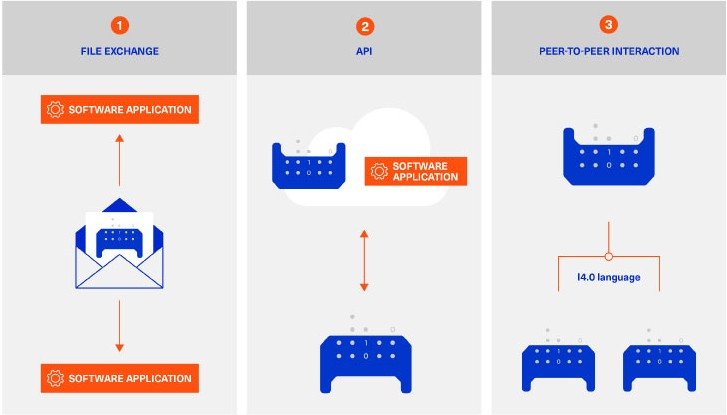
\includegraphics[width=12cm]{Images/AAS_Types.jpg}
    \caption{Types of Asset Administration Shells \cite{plattformI40_aas_part2}}
    \label{fig:AAS_Types}
\end{figure}

\newpage
\subsection{AAS Type3}
\label{subsec:aas_type3}
The \textit{type3} \ac{AAS} builds upon the capabilities of \textit{type2} \ac{AAS} by introducing a peer-to-peer network of \ac{AAS}s \cite{Sakurada2025_MAS_AAS_Type3}.
The \textit{type3} represents a more advanced and extended form of \ac{AAS}, 
acting as a decision-making entity that autonomously interacts with other \ac{AAS}s to exchange information and collaborate (e.g., through negotiation) \cite{Sakurada2025_MAS_AAS_Type3}.
The core idea of the Asset Administration Shell \ac{AAS} concept is that every industrial asset is represented by its own \ac{AAS}, 
thereby transforming the asset into an \ac{I4.0} component \cite{Sakurada2025_MAS_AAS_Type3}.
Because all \ac{AAS}s follow a unified, standardized structure and expose \ac{I4.0}-compliant interfaces, 
they enable seamless information provision and exchange across the entire lifecycle of an asset.
This standardization facilitates interoperability and real-time data sharing among heterogeneous assets, 
independent of manufacturer or application domain \cite{LOPEZ2023103859}.
In figure~\ref{fig:AAS_Type3_Concept}, the concept of \textit{type3} \ac{AAS} is illustrated.
\begin{figure}[ht]
    \centering
    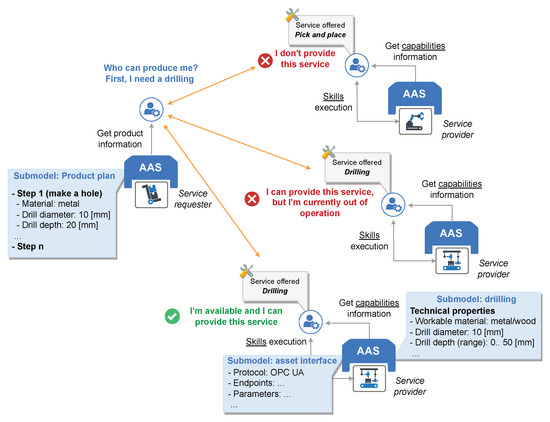
\includegraphics[width=12cm]{Images/type3_aas.jpg}
    \caption{Concept of Type3 AAS \cite{Sakurada2025_MAS_AAS_Type3}}
    \label{fig:AAS_Type3_Concept}
\end{figure}
Through their \ac{AAS} representations, assets are thus envisioned to autonomously collaborate, 
coordinate processes, and contribute to decentralized decision-making within industrial systems \cite{LOPEZ2023103859}.
However, such autonomous, intelligent, and cooperative behavior corresponds primarily to \ac{AAS} \textit{type3}, 
which unlike \ac{AAS} \textit{type1} and \textit{type2} remains comparatively underexplored and currently lacks dedicated specifications and comprehensive implementation guidelines \cite{Sakurada2025_MAS_AAS_Type3}.
The \textit{type3} \ac{AAS} revolves around three main requirements \cite{Sakurada2025_MAS_AAS_Type3} , \cite{LOPEZ2023103859}, \cite{vogel2021approach}, \cite{monostori2006agent}:
\begin{itemize}
    \item \textbf{Autonomy}: Each \ac{AAS} should operate independently, makin g decisions and executing actions without human intervention.
    \item \textbf{Intelligence}: \ac{AAS}s should possess cognitive capabilities, enabling them to learn from their environment, adapt to changes, and optimize their performance over time.
    \item \textbf{Collaboration}: \ac{AAS}s should be able to communicate and collaborate with other \ac{AAS}s, forming a network of interconnected agents that work together to achieve common goals.
\end{itemize}
The \textit{type3} is currently an area of active research and development,
with ongoing efforts to define its specifications and explore its potential applications in Industry 4.0 environments \cite{Sakurada2025_MAS_AAS_Type3}.
There is to be yet no standardized framework or guidelines for implementing \textit{type3} \ac{AAS},
making it a promising avenue for future exploration and innovation in the field of industrial automation and digitalization \cite{Sakurada2025_MAS_AAS_Type3}.

\subsection{Summary}
\label{subsec:aas_summary}

This section has introduced the \ac{AAS} as the standardized digital representation of industrial assets within the Industry 4.0 ecosystem. The key concepts covered include:

\begin{itemize}
    \item The \ac{AAS} meta-model, which defines the structure for representing assets through identifiable, self-describing information models that can be exchanged in \ac{XML}, \ac{JSON}, or \ac{RDF} formats.
    
    \item Submodels as modular components that encapsulate specific aspects of an asset, including properties, operations, events, and capabilities. Standardized submodel templates enable interoperability across different vendors and application domains.
    
    \item The classification of \ac{AAS} into three types based on their interaction capabilities: Type~1 (file exchange), Type~2 (API-based communication), and Type~3 (peer-to-peer proactive interaction).
    
    \item The requirements of \ac{Type3AAS}---autonomy, proactive behavior, and collaboration---which extend beyond the current specifications and require additional technologies to be realized.
\end{itemize}

Of particular relevance to this thesis is the \ac{Type3AAS}, which envisions assets as autonomous entities capable of proactive decision-making and peer-to-peer collaboration. However, as noted, the \ac{Type3AAS} currently lacks formal specifications and implementation guidelines. The standardized Operation element defined in the \ac{AAS} meta-model provides a potential interface for executing agent actions, yet this capability remains underutilized in existing implementations. The following sections introduce \ac{MAS} and the \ac{BDI} architecture as enabling technologies for realizing the proactive capabilities required by \ac{Type3AAS}.



%-------------------
\section{Multi-Agent Systems (MAS)}
\label{sec:mas}

The concept of autonomous agents and \ac{MAS} has emerged as a powerful paradigm for designing and implementing complex distributed systems that require autonomous behavior, coordination, and adaptability \cite{wooldridge2009introduction}. This section introduces the fundamental concepts of agents and \ac{MAS}, establishing the theoretical foundation for understanding their integration with \ac{AAS} to realize \ac{Type3AAS} capabilities.

\subsection{Agents and Their Properties}
\label{subsec:agents_properties}

An agent is commonly defined as ``a computer system that is situated in some environment, and that is capable of autonomous action in this environment in order to meet its design objectives'' \cite{wooldridge2009introduction}. Unlike conventional software components that execute predefined instructions in response to method calls, agents exhibit a higher degree of autonomy and environmental awareness.

According to \cite{wooldridge1995intelligent}, an intelligent agent possesses the following essential properties:

\begin{itemize}
    \item \textbf{Autonomy}: Agents operate without direct intervention from humans or other agents. They have control over their own actions and internal state, making independent decisions based on their goals and perceptions.
    
    \item \textbf{Reactivity}: Agents perceive their environment through sensors or data interfaces and respond in a timely manner to changes that occur in it. This enables agents to adapt to dynamic conditions.
    
    \item \textbf{Proactivity}: Beyond merely reacting to environmental changes, agents can exhibit goal-directed behavior by taking initiative. They can anticipate future states and act to achieve their objectives without external prompting.
    
    \item \textbf{Social Ability}: Agents can interact with other agents (and potentially humans) through some form of agent communication language to coordinate activities, negotiate, and cooperate toward shared or individual goals.
\end{itemize}

These properties distinguish agents from traditional software objects and make them particularly suitable for applications requiring autonomous decision-making and adaptive behavior, such as the proactive capabilities envisioned for \ac{Type3AAS}.

\subsection{Multi-Agent Systems}
\label{subsec:mas_definition}

A \ac{MAS} is a system composed of multiple interacting agents that work together within a shared environment \cite{wooldridge2009introduction}. Each agent in a \ac{MAS} has its own goals, capabilities, and knowledge, and the collective behavior of the system emerges from the interactions among individual agents.

\ac{MAS} offer several advantages over centralized systems \cite{leitao2016smart}:

\begin{itemize}
    \item \textbf{Decentralization}: There is no single point of control or failure. Each agent operates autonomously, making the system more robust and resilient to local failures.
    
    \item \textbf{Scalability}: New agents can be added to the system without requiring fundamental changes to existing agents, allowing the system to grow incrementally.
    
    \item \textbf{Flexibility}: Agents can dynamically reorganize and adapt their interactions in response to changing requirements or environmental conditions.
    
    \item \textbf{Modularity}: Each agent encapsulates specific functionality, promoting separation of concerns and facilitating maintenance and evolution of the system.
\end{itemize}

These characteristics align closely with the requirements of modern manufacturing systems, where flexibility, adaptability, and resilience are essential to cope with increasing product variety, shorter product lifecycles, and unpredictable disruptions \cite{leitao2016smart}.

\subsection{Agent Architectures}
\label{subsec:agent_architectures}

Agent architectures define the internal structure of agents and how they process perceptions to generate actions. Three main categories of agent architectures have been identified in the literature \cite{wooldridge2009introduction}:

\textbf{Reactive Architectures} implement a direct mapping from perceptions to actions without maintaining an internal model of the world. These architectures, such as the subsumption architecture proposed by Brooks \cite{brooks1986robust}, are computationally efficient and provide fast responses but lack the ability to reason about complex goals or plan ahead.

\textbf{Deliberative Architectures} maintain an explicit symbolic model of the world and use logical reasoning to determine appropriate actions. These architectures can handle complex planning tasks but may be computationally expensive and slow to respond to rapidly changing environments.

\textbf{Hybrid Architectures} combine reactive and deliberative components to balance responsiveness with reasoning capabilities. A typical hybrid architecture consists of multiple layers: a reactive layer for immediate responses, a deliberative layer for planning and reasoning, and a coordination layer that mediates between them. The \ac{BDI} architecture, discussed in Section \ref{sec:bdi}, represents a well-established hybrid approach that provides both reactive capabilities and goal-directed reasoning.

\subsection{Agent Communication}
\label{subsec:agent_communication}

Communication is fundamental to \ac{MAS}, enabling agents to share information, coordinate activities, and negotiate agreements. The \ac{FIPA} has established standards for agent communication that are widely adopted in industrial applications \cite{fipa2002acl}.

The FIPA \ac{ACL} defines a set of performatives (communicative acts) that specify the intended meaning of messages exchanged between agents. Common performatives include:

\begin{itemize}
    \item \texttt{INFORM}: Used to share information or beliefs with other agents
    \item \texttt{REQUEST}: Used to ask another agent to perform an action
    \item \texttt{PROPOSE}: Used to make a proposal during negotiation
    \item \texttt{ACCEPT-PROPOSAL} / \texttt{REJECT-PROPOSAL}: Used to respond to proposals
    \item \texttt{CFP} (Call for Proposals): Used to initiate a negotiation or auction
\end{itemize}

These standardized performatives enable interoperability between agents developed using different frameworks and facilitate the implementation of coordination protocols such as the Contract Net Protocol \cite{smith1980contract}, which is commonly used for task allocation in manufacturing systems.

\subsection{Agent Coordination and Cooperation}
\label{subsec:agent_coordination}

In \ac{MAS}, agents must coordinate their activities to achieve common goals and avoid conflicts. Several coordination mechanisms have been developed \cite{wooldridge2009introduction}:

\textbf{Contract Net Protocol}: A market-based mechanism where a manager agent announces a task, receives bids from contractor agents, and awards the contract to the most suitable bidder. This protocol is widely used in manufacturing for dynamic task allocation \cite{smith1980contract}.

\textbf{Auction-Based Coordination}: Agents participate in auctions to acquire resources or tasks. Different auction types (English, Dutch, sealed-bid) offer trade-offs between communication overhead and optimality of allocation.

\textbf{Negotiation}: Agents engage in a dialogue to reach mutually acceptable agreements. Negotiation is essential when agents have conflicting interests but need to cooperate for mutual benefit.

\textbf{Organizational Structures}: Agents can be organized into hierarchies, teams, or coalitions with defined roles and responsibilities. Organizational models such as Moise+ \cite{hubner2007moise} provide formal frameworks for specifying agent organizations.

\subsection{Industrial Agents}
\label{subsec:industrial_agents}

The application of agent technology in industrial settings has given rise to the concept of industrial agents, which are agents specifically designed for manufacturing and production environments \cite{leitao2016smart}. Industrial agents typically operate within a two-layered architecture as illustrated in Figure \ref{fig:industrial_agent_layers}:
\begin{figure}[ht]
    \centering
    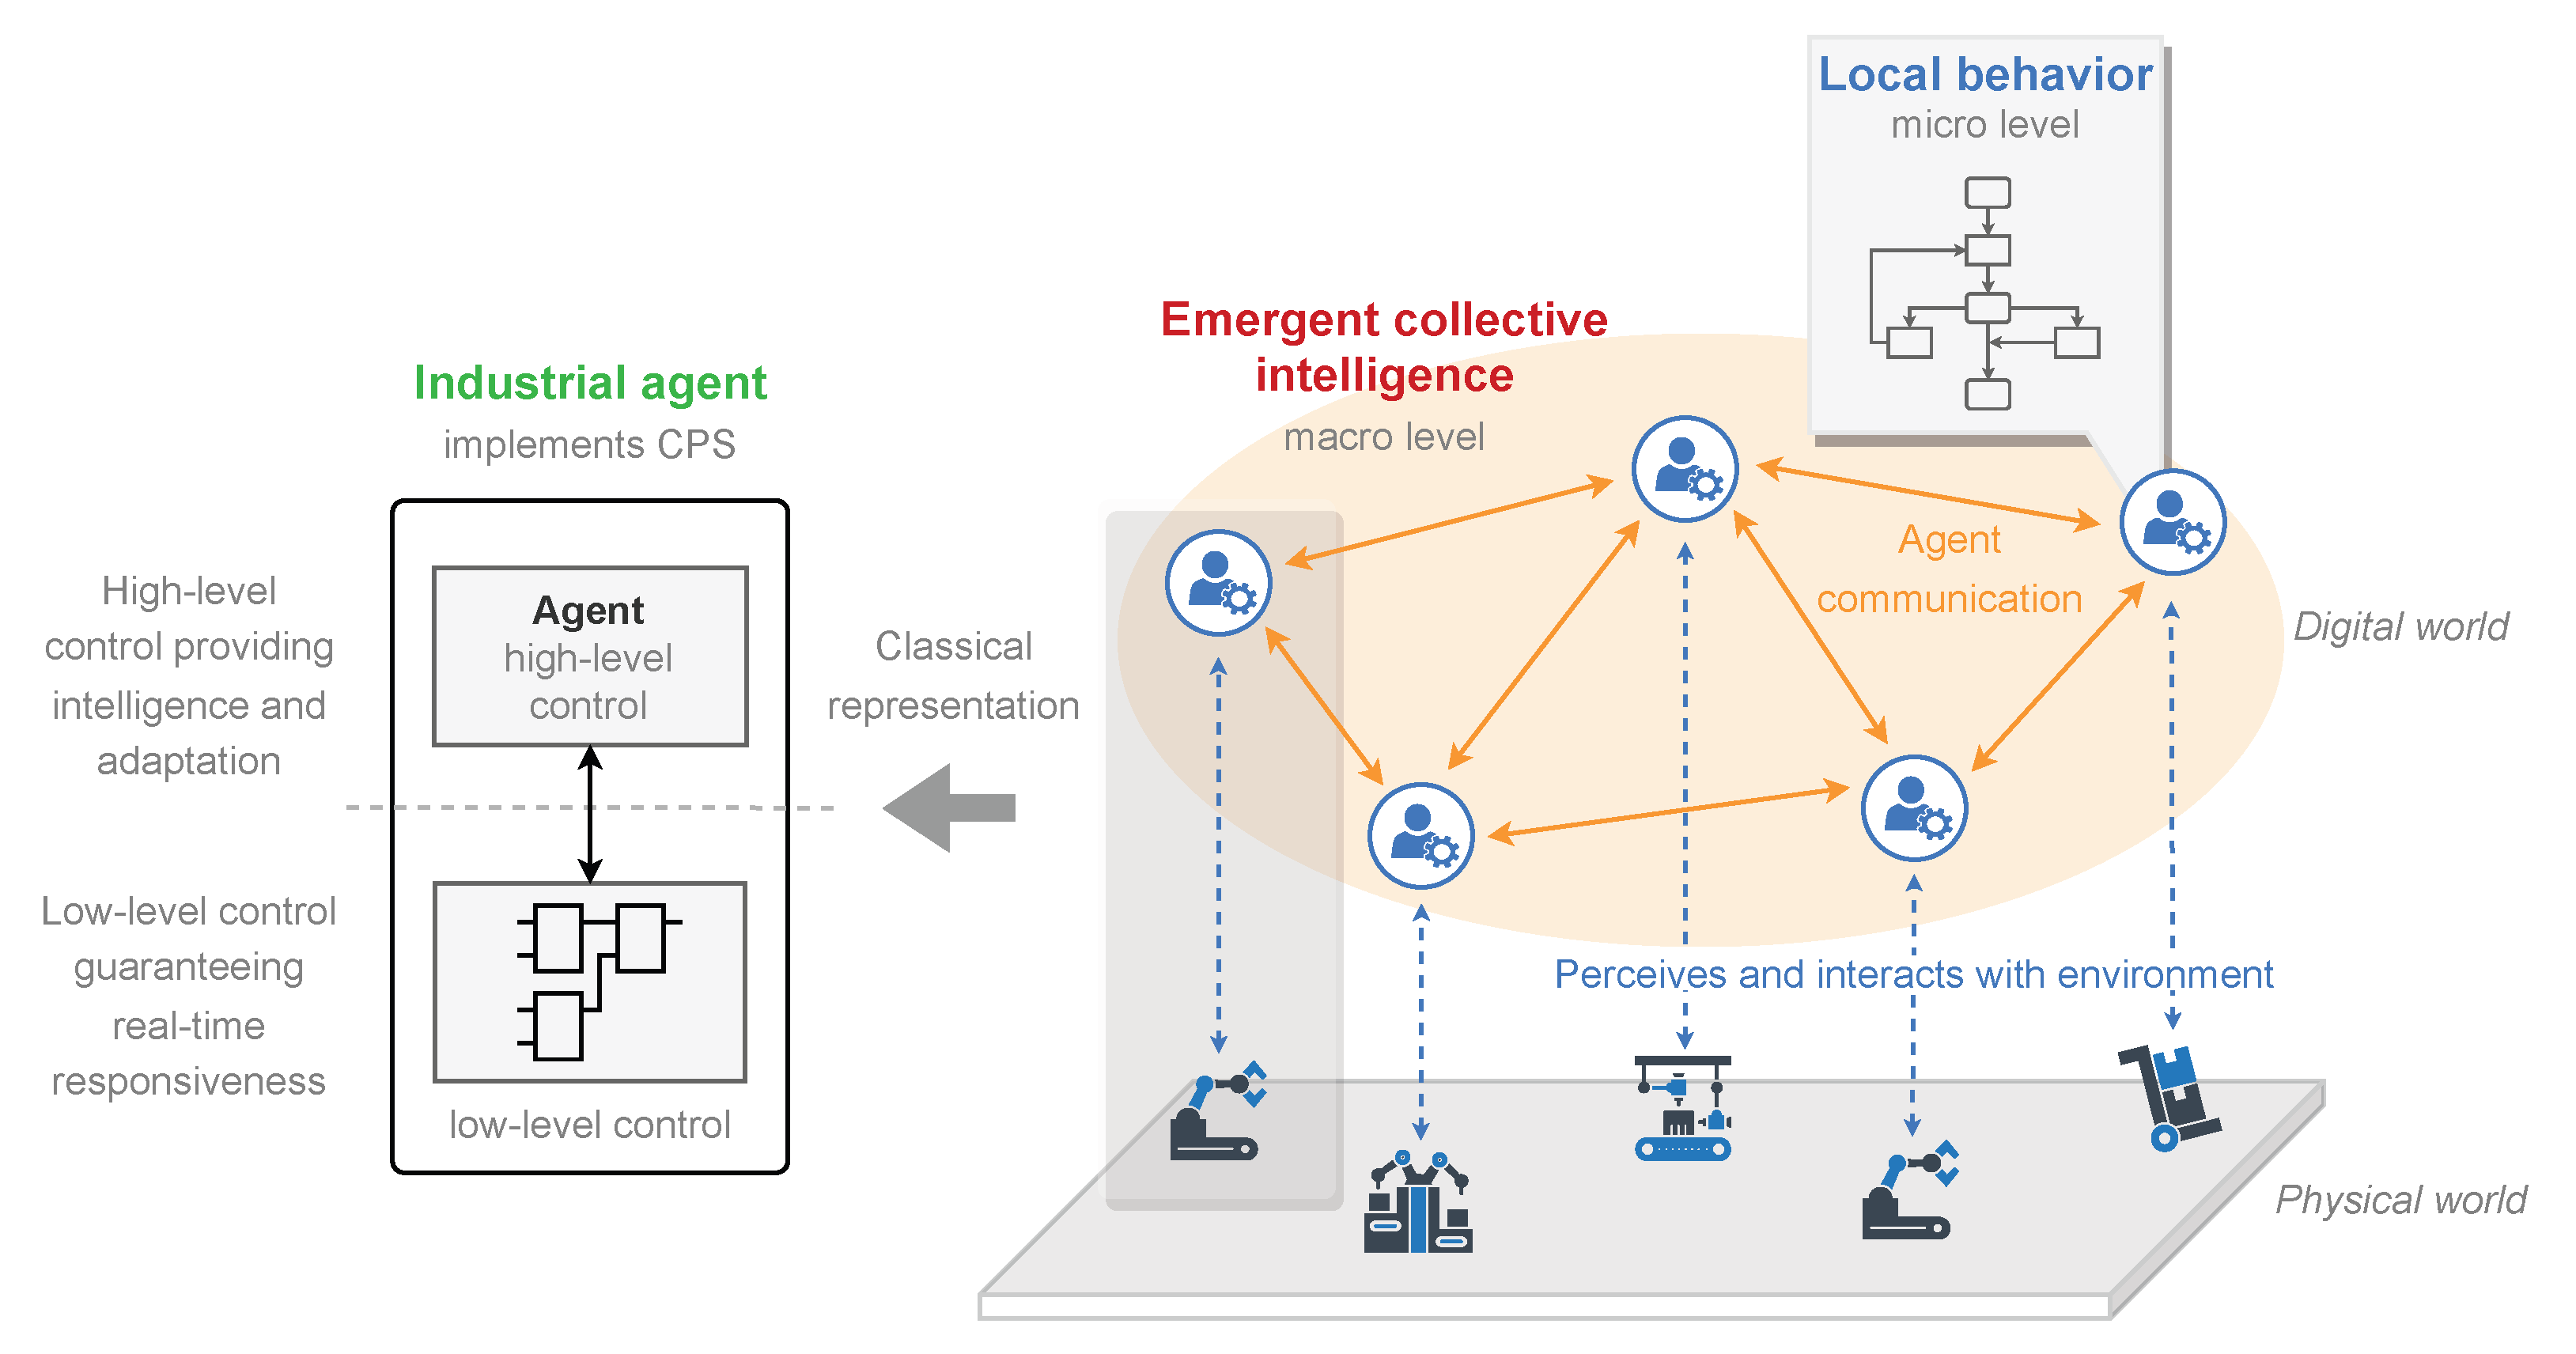
\includegraphics[width=12cm]{Images/Industrial_agent_approach.png}
    \caption{Industrial Agent Layers \cite{leitao2021recommendation}}
    \label{fig:industrial_agent_layers}
\end{figure}

\begin{itemize}
    \item \textbf{\ac{LLC}}: This layer handles real-time control of physical assets, including sensor monitoring, actuator control, and safety functions. It is typically implemented using \ac{PLC}s or industrial PCs with real-time operating systems.
    
    \item \textbf{\ac{HLC}}: This layer implements the agent logic, including decision-making, coordination, and communication with other agents. It provides intelligence and adaptability while delegating time-critical operations to the LLC layer.
\end{itemize}

This separation allows agents to leverage the reliability and determinism of industrial control systems while adding intelligent, adaptive behavior through the agent layer. The interface between these layers can be implemented using industrial communication standards such as \ac{OPC UA}, which aligns well with the communication capabilities specified for \ac{AAS} \cite{leitao2021recommendation}.

Industrial agents have been successfully applied in various manufacturing scenarios, including flexible manufacturing systems, supply chain management, and production scheduling \cite{leitao2016smart}. Their ability to operate autonomously, coordinate with peers, and adapt to changing conditions makes them natural candidates for implementing the proactive behavior required by \ac{Type3AAS}.

\subsection{Summary}
\label{subsec:mas_summary}

This section has introduced the fundamental concepts of agents and \ac{MAS}, including agent properties, architectures, communication, and coordination mechanisms. The key characteristics of agents autonomy, reactivity, proactivity, and social ability align directly with the requirements identified for \ac{Type3AAS}: autonomous operation, intelligent decision-making, and collaborative interaction. Industrial agents provide a proven approach for deploying agent technology in manufacturing environments, with established patterns for integrating intelligent behavior with real-time control systems. The following section examines the \ac{BDI} architecture, which provides a specific model for implementing rational, goal-directed agents suitable for \ac{Type3AAS} applications.



\newpage
\section{BDI (Belief-Desire-Intention) Approach}
\label{sec:bdi}
The \ac{BDI} architecture represents one of the most influential and well-established models for implementing rational agents capable of autonomous decision-making \cite{wooldridge1995intelligent}. Originally rooted in the philosophical theory of human practical reasoning developed by Bratman \cite{bratman1987intention}, the \ac{BDI} model has been successfully adapted into a computational framework for programming intelligent agents that exhibit goal-directed behavior \cite{rao1995bdi}.
\subsection{Foundations of the BDI Model}

The \ac{BDI} architecture is grounded in three core mental attitudes that guide an agent's reasoning and behavior \cite{bratman1987intention}:

\begin{itemize}
    \item \textbf{Beliefs}: Represent the agent's knowledge about itself, other agents, and its environment. Beliefs are informational states that the agent holds to be true based on its perceptions and prior knowledge. In the context of \ac{AAS}, beliefs can be derived from submodel data, sensor readings, or information received from other I4.0 components.
    
    \item \textbf{Desires}: Represent the goals or objectives that the agent would like to achieve. Desires are motivational states that drive the agent's behavior. For a \ac{Type3AAS}, desires might include optimizing production throughput, minimizing energy consumption, or completing manufacturing orders.
    
    \item \textbf{Intentions}: Represent the desires that the agent has committed to pursue. Intentions are deliberative states that the agent has decided to act upon, providing a form of commitment that ensures persistence in goal pursuit while allowing for reconsideration when circumstances change significantly.
\end{itemize}

The interplay between these three attitudes enables agents to reason about their goals, select appropriate plans, and execute actions in a rational manner \cite{rao1995bdi}. This separation of concerns allows for a clear distinction between what the agent knows (beliefs), what it wants to achieve (desires), and what it is currently trying to do (intentions).

\subsection{The BDI Reasoning Cycle}

A \ac{BDI} agent operates through a continuous reasoning cycle that processes perceptions from the environment and generates actions \cite{bordini2007programming}. The typical reasoning cycle consists of the following steps:

\begin{enumerate}
    \item \textbf{Perception}: The agent perceives changes in its environment and updates its belief base accordingly.
    
    \item \textbf{Belief Revision}: Based on new perceptions, the agent revises its beliefs to maintain consistency with the current state of the world.
    
    \item \textbf{Option Generation}: The agent generates possible options (potential desires) based on its current beliefs and existing goals.
    
    \item \textbf{Deliberation}: The agent deliberates over the available options and selects which goals to commit to as intentions.
    
    \item \textbf{Plan Selection}: For each intention, the agent selects an appropriate plan from its plan library that can achieve the intended goal given current beliefs.
    
    \item \textbf{Action Execution}: The agent executes the next action in the selected plan, which may affect the environment and trigger new perceptions.
\end{enumerate}

This cycle enables \ac{BDI} agents to exhibit both reactive behavior (responding to environmental changes) and proactive behavior (pursuing long-term goals), which aligns with the requirements of \ac{Type3AAS} \cite{wooldridge1995intelligent}.
\begin{figure}[ht]
    \centering
    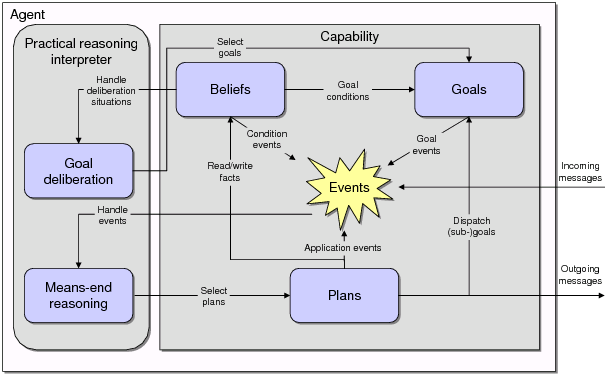
\includegraphics[width=12cm]{Images/BDI_concept.png}
    \caption{BDI Reasoning Cycle \cite{Pokahr2007_JadexConcepts}}
    \label{fig:bdi_reasoning_cycle}
\end{figure}

\newpage
\subsection{BDI for Industrial and Cyber-Physical Systems}

The application of \ac{BDI} agents in industrial settings has gained significant attention due to their ability to handle complex decision-making in dynamic environments \cite{leitao2021recommendation}. In the context of \ac{CPS} and Industry 4.0, \ac{BDI} agents offer several advantages:

\begin{itemize}
    \item \textbf{Autonomy}: \ac{BDI} agents can operate independently, making decisions without constant human supervision, which is essential for autonomous manufacturing systems.
    
    \item \textbf{Adaptability}: The belief revision mechanism allows agents to adapt to changing conditions in real-time, responding to unexpected events such as machine failures or order changes.
    
    \item \textbf{Explainability}: The explicit representation of beliefs, desires, and intentions provides a transparent model of agent behavior, facilitating debugging, validation, and trust in autonomous systems \cite{yan2025multi}.
    
    \item \textbf{Goal-Directed Behavior}: The intention-based commitment strategy ensures that agents persistently pursue their goals while maintaining the flexibility to reconsider when necessary.
\end{itemize}

\newpage

\subsection{Summary}

The \ac{BDI} architecture provides a well-founded theoretical and practical framework for implementing rational agents capable of autonomous decision-making. Its clear separation of beliefs, desires, and intentions enables transparent reasoning processes that are essential for industrial applications where explainability and trust are paramount. The availability of mature programming frameworks such as Jason and JaCaMo facilitates the development of \ac{BDI}-based multi-agent systems. When integrated with the \ac{AAS} concept, \ac{BDI} agents can leverage standardized asset information and communication interfaces to realize the proactive, collaborative behavior envisioned for \ac{Type3AAS}. This integration forms the conceptual basis for the approach proposed in this thesis.

\section{Software Frameworks and Platforms}
\label{sec:software frameworks and platforms}

The realization of \ac{Type3AAS} requires not only theoretical foundations but also practical software tools and frameworks. This section reviews the current state of available frameworks for implementing \ac{AAS}, \ac{MAS}, and \ac{BDI} agents, providing the technical context for the implementation decisions made in this thesis.



\subsection{Asset Administration Shell Frameworks}
\label{subsec:aas_frameworks}
Several open-source and commercial frameworks have emerged to support the development and deployment of \ac{AAS} implementations. The most prominent frameworks include:

\textbf{Eclipse BaSyx} is an open-source middleware platform developed under the Eclipse Foundation that provides a comprehensive implementation of the \ac{AAS} specification \cite{2023basyx}. BaSyx offers:
\begin{itemize}
    \item Complete implementation of the \ac{AAS} meta-model and API specification
    \item Support for both Type~1 (file-based) and Type~2 (API-based) \ac{AAS}
    \item Registry and discovery services for \ac{AAS} components
    \item Integration capabilities with industrial protocols (\ac{OPC UA}, \ac{MQTT}, \ac{HTTP},\ac{REST})
    \item Modular architecture allowing selective deployment of components
\end{itemize}
BaSyx is widely adopted in research and industry due to its open-source nature and active community support. However, it does not natively support \ac{Type3AAS} capabilities such as autonomous decision-making or proactive behavior.

\textbf{\ac{FAAAST}} is another open-source framework that focuses on ease of use and rapid prototyping \cite{2023faast}. It provides:
\begin{itemize}
    \item Lightweight implementation suitable for resource-constrained environments
    \item Support for multiple serialization formats (JSON, XML, RDF)
    \item Built-in synchronization with asset data sources
    \item Extensible architecture for custom functionality
\end{itemize}

\textbf{AASX Package Explorer} is a desktop application developed by the \ac{IDTA} for creating, viewing, and editing \ac{AAS} packages \cite{2023aasxexplorer}. While primarily a development and visualization tool rather than a runtime framework, it serves as an important reference implementation and is commonly used for:
\begin{itemize}
    \item Creating and validating \ac{AAS} models
    \item Importing and exporting \ac{AAS} packages in standardized formats
    \item Visualizing submodel structures and relationships
    \item Testing interoperability between different \ac{AAS} implementations
\end{itemize}

\textbf{Limitations for Type~3 AAS}: All current \ac{AAS} frameworks focus on Type~1 and Type~2 functionality. None provide native support for the autonomous, proactive behavior required by \ac{Type3AAS}. This gap motivates the integration with agent-based technologies explored in this thesis.


\subsection{Multi-Agent System Frameworks}
\label{subsec:mas_frameworks}

Several mature frameworks exist for developing \ac{MAS}, each with different design philosophies and target applications:

\textbf{\ac{JADE}} is one of the most widely used \ac{MAS} platforms, providing a FIPA-compliant infrastructure for agent development in Java \cite{2023jade}. Key features include:
\begin{itemize}
    \item Full compliance with \ac{FIPA} specifications for agent communication
    \item Distributed agent platform with support for multiple containers
    \item Built-in agent management and directory services
    \item Graphical tools for debugging and monitoring agent behavior
    \item Behavior-based agent programming model
\end{itemize}
\ac{JADE} has been extensively used in industrial applications and research projects. However, its behavior-based programming model does not directly support cognitive agent architectures such as \ac{BDI}.

\textbf{\ac{SPADE}} is a modern \ac{MAS} platform built on Python and \ac{XMPP} \cite{2023spade}. SPADE offers:
\begin{itemize}
    \item Asynchronous agent execution using Python's asyncio
    \item \ac{XMPP}-based communication providing robust, scalable messaging
    \item Web-based interface for agent monitoring
    \item Flexible behavior system with support for cyclic, one-shot, and finite-state behaviors
    \item Easy integration with Python's extensive ecosystem of libraries
\end{itemize}
\ac{SPADE}'s use of \ac{XMPP} provides advantages for industrial deployments, including message persistence, presence detection, and established security mechanisms. Its Python foundation also facilitates rapid prototyping and integration with data science tools.

\textbf{\ac{JADEX}} extends JADE with \ac{BDI} reasoning capabilities, combining JADE's robust infrastructure with cognitive agent programming \cite{2023jadex}. JADEX supports:
\begin{itemize}
    \item \ac{BDI} agent development using \ac{XML}-based agent definitions
    \item Integration with JADE's communication infrastructure
    \item Goal-oriented programming with automatic plan selection
    \item Active components model for service-oriented architectures
\end{itemize}

\subsection{Framework selection considerations}
The selection of appropriate frameworks for implementing \ac{Type3AAS} depends on several factors:

\begin{itemize}
    \item \textbf{AAS Compliance}: The \ac{AAS} framework must support the current specification, including submodel operations and standardized APIs.
    
    \item \textbf{Agent Architecture Support}: For \ac{BDI}-based implementations, the \ac{MAS} framework should either natively support \ac{BDI} or allow integration with \ac{BDI} reasoning engines.
    
    \item \textbf{Communication Capabilities}: Industrial deployments require robust, scalable communication mechanisms that can handle asynchronous messaging and potential network disruptions.
    
    \item \textbf{Integration Flexibility}: The ability to connect \ac{AAS} and \ac{MAS} components through well-defined interfaces is essential for realizing bidirectional integration.
    
    \item \textbf{Development Ecosystem}: Practical considerations such as documentation quality, community support, and available tooling influence development efficiency.
\end{itemize}

Tables~\ref{tab:aas_framework_comparison},\ref{tab:mas_framework_comparison} provides a comparative overview of the discussed frameworks.

\begin{table}[ht]
\centering
\caption{Comparison of Asset Administration Shell frameworks}
\label{tab:aas_framework_comparison}
\begin{tabular}{>{\raggedright}p{3.5cm} >{\centering}p{2.5cm} >{\centering}p{3cm} >{\centering\arraybackslash}p{4cm}}
\toprule
\rowcolor{headerblue}
\textcolor{white}{Framework} & \textcolor{white}{Language} & \textcolor{white}{AAS Types} & \textcolor{white}{Communication} \\
\midrule
Eclipse BaSyx & Java / Python & Type 1, Type 2 & HTTP/REST, MQTT, OPC UA \\
\rowcolor{lightgray}
FA³ST Service & Java & Type 1, Type 2 & HTTP/REST, OPC UA \\
AASX Package Explorer & C\# & Type 1 & File-based (AASX) \\
\bottomrule
\end{tabular}
\end{table}

% ============================================
% Table 2: MAS and BDI Frameworks
% ============================================

\begin{table}[ht]
\centering
\caption{Comparison of Multi-Agent System and BDI frameworks}
\label{tab:mas_framework_comparison}
\begin{tabular}{>{\raggedright}p{3cm} >{\centering}p{2.5cm} >{\centering}p{2.5cm} >{\centering\arraybackslash}p{4cm}}
\toprule
\rowcolor{headerblue}
\textcolor{white}{Framework} & \textcolor{white}{Language} & \textcolor{white}{BDI Support} & \textcolor{white}{Communication} \\
\midrule
JADE & Java & No (ext.) & FIPA \ac{ACL} \\
\rowcolor{lightgray}
SPADE & Python & Extension (spade-bdi) & \ac{XMPP} \\
JADEX & Java/\ac{XML} & Yes (native) & FIPA \ac{ACL} \\
\bottomrule
\end{tabular}
\end{table}
\subsection{Summary}
\label{subsec:frameworks_summary}

This section has reviewed the current landscape of software frameworks for \ac{AAS},
\ac{MAS}, and \ac{BDI} agent development. 
While mature frameworks exist for each domain individually, 
no single framework provides integrated support for 
\ac{Type3AAS} implementations. 
\ac{AAS} frameworks such as Eclipse BaSyx offer comprehensive support for Type~1 and Type~2 functionality but lack autonomous behavior capabilities. 
\ac{MAS} frameworks provide the agent infrastructure needed for autonomy and collaboration, with platforms like SPADE offering modern, asynchronous communication.
This fragmented landscape necessitates a custom integration approach, which is developed in subsequent chapters of this thesis.


\newpage
\section{Integration of AAS with MAS}

\label{sec:aas_mas_integration}

The preceding sections have established the foundational concepts of \ac{AAS} as standardized digital representations of industrial assets, \ac{MAS} as a paradigm for autonomous and collaborative systems, and the \ac{BDI} architecture as a model for goal-directed agent behavior. This section examines how these concepts can be combined to realize \ac{Type3AAS} implementations, reviewing existing approaches and identifying the research gaps that this thesis addresses.

As discussed in Section~\ref{subsec:aas_type3}, the requirements of \ac{Type3AAS} autonomy, proactive behavior, and collaboration align closely with the core properties of agents identified in Section~\ref{subsec:agents_properties}. This alignment has motivated several research efforts to implement \ac{Type3AAS} using \ac{MAS} concepts. Table~\ref{tab:aas_type3_mas_implementations} summarizes the key approaches found in the literature.




\ac{MAS} represent a decentralized approach to problem-solving,
by distributing tasks and responsibilities among multiple agents autonomously working towards common objectives,
on the contrary of traditional monolithic systems where a single entity controls the entire system\cite{leitao2016smart}.
There are several attempts to implement \textit{type3} \ac{AAS} based on \ac{MAS} concepts.
Those attempts are summarized in the table~\ref{tab:aas_type3_mas_implementations}.

\begin{longtable}{>{\raggedright\bfseries}p{3cm} >{\raggedright}p{5cm} >{\raggedright\arraybackslash}p{5cm}}
\caption{Summary of AAS Type 3 implementations based on MAS concepts} 
\label{tab:aas_type3_mas_implementations} \\
\toprule
\rowcolor{headerblue}
\textcolor{white}{Reference} & \textcolor{white}{Approach} & \textcolor{white}{Key Features} \\
\midrule
\endfirsthead

% Header for continuation pages
\multicolumn{3}{c}{\tablename\ \thetable{} -- continued from previous page} \\
\toprule
\rowcolor{headerblue}
\textcolor{white}{Reference} & \textcolor{white}{Approach} & \textcolor{white}{Key Features} \\
\midrule
\endhead

% Footer for pages that continue
\midrule
\multicolumn{3}{r}{\textit{Continued on next page}} \\
\endfoot

% Final footer
\bottomrule
\endlastfoot

% Table content - ADD YOUR ROWS HERE
\rowcolor{lightgray}
Vogel-Heuser et al. (2021) \cite{vogel2021approach} & Approach using AAS as knowledge base for the agents & Demonstrated on a stack-crane system  \\
Sakurada et al. (2022) \cite{sakurada2022engineering} & Method for implementing \ac{AAS}s using \ac{MAS} & Decentralized production control, peer-to-peer communication, demonstrated on simulation \\
\rowcolor{lightgray}
Siatras et al. (2024) \cite{siatras2024production} & Agents operate in \ac{MAS} to solve scheduling problems where the \ac{AAS} provide production and agent information & Demonstrated on real production line \\
Sidorenko et al. (2023) \cite{sidorenko2023mas4ai}& A framework that combines \ac{MAS} with \ac{AAS} to enable human-centered manufacturing & Demonstrated on robot with human collaboration \\
\rowcolor{lightgray}
Jungbluth et al. (2022) \cite{jungbluth2022dynamic} & Modeling \ac{AAS} submodels for resource and production agents   & Demonstrated on an assembly line \\

\end{longtable}

The literature shows consensus that submodels serve as standardized knowledge sources for agents, capturing asset-related information in formats accessible to both humans and machines \cite{Sakurada2025_MAS_AAS_Type3}. Agents leverage these submodels to support decision-making and enrich their knowledge bases. Standardized submodels, such as the Control Component Instance \cite{idta2023controlcomponent}, Asset Interfaces Description \cite{industrial2024idta}, and Time-Series Data \cite{industrial2023idta}, describe the skills offered by an asset, the methods for interfacing with it, and the mechanisms for managing operational data.

Beyond standardized submodels, custom submodels can be defined to address specific application requirements and represent agent-specific information, such as agent behaviors, decision-making strategies, or interaction protocols, thereby enhancing transparency and understanding of agent capabilities \cite{Sakurada2025_MAS_AAS_Type3}.

The review further reveals that communication capabilities represent one of the most emphasized and valuable features of agents. This inherent characteristic positions agents as powerful enablers for achieving the decentralized and collaborative interactions particularly through negotiation strategies envisioned in \ac{Type3AAS} implementations \cite{Sakurada2025_MAS_AAS_Type3}.


\subsection{Critical Analysis of Existing Approaches}
\label{subsec:critical_analysis}

The existing approaches to implementing \ac{Type3AAS} based on \ac{MAS} concepts, as summarized in Table \ref{tab:aas_type3_mas_implementations}, demonstrate promising directions but also reveal significant limitations that motivate further research.

\subsubsection{Strengths of Current Approaches}

Several positive aspects emerge from the reviewed literature. First, there is a clear consensus on the architectural separation between the \ac{AAS} as a standardized knowledge repository and the agent as an autonomous decision-making entity \cite{vogel2021approach, sakurada2022engineering}. This separation allows each component to leverage its respective strengths: the \ac{AAS} provides interoperability and standardized data access, while agents contribute autonomous behavior and coordination capabilities.

Second, the use of submodels as structured knowledge sources for agents has proven effective across multiple implementations \cite{jungbluth2022dynamic, Sakurada2025_MAS_AAS_Type3}. Standardized submodels such as the Control Component Instance \cite{idta2023controlcomponent} provide a common vocabulary for describing asset capabilities, enabling agents to interpret and reason about heterogeneous assets in a uniform manner.

Third, several approaches have successfully demonstrated decentralized production control through agent negotiation and collaboration \cite{sakurada2022engineering, siatras2024production}. This validates the fundamental premise that \ac{MAS} can enable the peer-to-peer interactions envisioned for \ac{Type3AAS}.

\subsubsection{Limitations and Open Challenges}

Despite these advances, the reviewed approaches exhibit several common limitations:

\textbf{Unidirectional AAS Usage.} Current approaches primarily use the \ac{AAS} as a passive, read-only data source. Agents retrieve information from submodels to inform their decisions, but the potential of the \ac{AAS} as an interface for executing actions remains largely unexplored. The \ac{AAS} specification defines Operations as executable functions that can be invoked synchronously or asynchronously \cite{plattformI40_aas_part2}, yet existing implementations do not fully leverage this capability for agent action execution.

\textbf{Lack of Standardized Submodels for Agent Behavior.} While standardized submodels exist for describing asset capabilities (e.g., Control Component Instance \cite{idta2023controlcomponent}) and interfaces (e.g., Asset Interfaces Description \cite{industrial2024idta}), there are no established submodel templates specifically designed to represent agent-related information such as goals, desires, or behavioral parameters. This limits the transparency and interoperability of agent-based \ac{Type3AAS} implementations.

\textbf{Validation Predominantly in Simulation.} The majority of approaches have been validated only in simulated environments \cite{sakurada2022engineering} or on simplified laboratory setups \cite{vogel2021approach}. While simulation provides a controlled environment for initial validation, it does not fully capture the complexities, uncertainties, and real-time constraints of actual industrial deployments.

\textbf{Lack of Standardized Agent-AAS Integration Patterns.} Each reviewed approach implements the integration between agents and \ac{AAS} in a different manner, with no established design patterns or reference architectures. This heterogeneity hinders reusability, comparison, and adoption across different industrial contexts.

\textbf{Missing Connection Between AAS Operations and Agent Actions.} A critical gap exists in how agent intentions are translated into standardized \ac{AAS} operations. Current implementations typically use proprietary interfaces for agent-asset interaction, bypassing the standardized Operation interface defined in the \ac{AAS} specification. This undermines the interoperability benefits that the \ac{AAS} standard aims to provide.

\subsection{Addressed Research Gap}

This thesis addresses the identified limitations by proposing a systematic integration of \ac{AAS} with \ac{BDI}-based agents that fully leverages the \ac{AAS} standard. Specifically, this work contributes:

\begin{enumerate}
    \item \textbf{Bidirectional AAS Integration}: Rather than using the \ac{AAS} solely as a data source, this thesis proposes a bidirectional integration where agents both read from submodels (to form beliefs) and invoke Operations (to execute intentions). This approach fully utilizes the capabilities specified in the \ac{AAS} standard, enabling agents to interact with assets through standardized interfaces rather than proprietary solutions.
    
    \item \textbf{Foundational Submodels for Proactive Behavior}: This work defines submodel structures specifically designed to support agent-based \ac{Type3AAS} implementations. These submodels represent goals, capabilities, and behavioral parameters that enable proactive decision-making while maintaining compliance with the \ac{AAS} meta-model. This contribution addresses the lack of standardized templates for agent-related information.
    
    \item \textbf{Proof-of-Concept with Production Resources}: The proposed approach is validated through a concrete use case involving drill machines as production resources. This demonstration shows the feasibility of implementing \ac{BDI}-based \ac{Type3AAS} in a realistic production scenario, moving beyond purely simulated environments to a more practical validation context.
\end{enumerate}

By addressing these gaps, this thesis aims to advance the state of the art toward truly interoperable, proactive I4.0 components that leverage the full potential of the \ac{AAS} standard while benefiting from the autonomous capabilities provided by agent technology.
